\documentclass[12pt,a4paper]{report}
\usepackage[onehalfspacing]{setspace}
\usepackage[a4paper, total={6in, 10in}]{geometry}
\usepackage[utf8]{inputenc}
\usepackage{graphicx}
\usepackage{wrapfig}
\usepackage{booktabs}
\usepackage{amsmath}
\usepackage{hyperref}
\usepackage{float}
\usepackage{pgfplots}
\usepackage{subcaption}
\graphicspath{{img}}
\usepackage{algorithm} 
\usepackage{algpseudocode} 
\usepackage{amsmath,amsfonts}
\usepackage{listings}
\usepackage{minted}
\usepackage{xcolor}
\usepackage{listings}
\usepackage{xparse}
\usepackage{soul}
\usepackage{minted}
\usepackage{etoolbox}
\patchcmd{\thebibliography}{\chapter*}{\section*}{}{}

%%%%%% Bibliography %%%%%%
% Replace "sample" in the \addbibresource line below with the name of your .bib file.
\usepackage[style=ieee, 
citestyle=numeric-comp,
sorting=none]{biblatex}


\addbibresource{mybib.bib}

\title{K-Nearest Neighbors(KNN)}
\author{Yohannis Kifle Telila}
\date{October 2021}

\pgfplotsset{compat=1.18}
\begin{document}
\begin{titlepage}
\begin{figure}[t]
    \centering
\includegraphics[width=0.4\textwidth]{images/cherubino.eps}
\end{figure}

\begin{center}
    \textbf{University of Pisa\\Department of Computer Science}
    \vspace{15mm}
    \\
    {\huge{Tweet Sentiment Analysis using Kafka and Spark : Elon Musk use case}}\\
    \vspace{5mm}
    \large{Yohannis Kifle Telila} \\
    \vspace{2mm}
    \large{Student ID : \textbf{621821} }
\end{center}

\vspace{20mm}
\begin{center}
    {\large Distributed Enabling Platforms - 534AA\\Academic year 2021/2022}
\end{center}
\vspace{36mm}
\end{titlepage}

\tableofcontents
\pagebreak

\chapter{Introduction}
\section{Problem description}

In recent years, social media websites have turned into a source of a wide range of information. This is due to the nature of social media, which allows users to generate real-time data, such as commenting about their perspectives on a range of topics, debate current events, and express emotions for topics or trending debates. Twitter, one of a social media platform which is estimated to have about 396.5 million monthly active users and these users create approximately 867 million tweets a day\cite{twitterStat}. These figures reflect Twitter's worldwide reach and potential effect globally.

Sentiment analysis (also known as opinion mining) is a natural language processing (NLP) approach for determining if statement is positive, negative, or neutral. Sentiment analysis can be performed for different purposes. For instance, Sentiment analysis is essential tool to detect and understand customer feelings\cite{DBLP:journals/corr/abs-1709-07434}. Companies that use these tool can understand how customers feels about their product and improve their product or service. However, the sheer amount and speed of Twitter's streaming data poses a significant technical hurdle. To process these amount of data we need a system  that is capable of horizontally scalable. Furthermore, the volume and the velocity of these tweets could vary in time. For such unpredictable and flexible environment we need a system that is fast, fault-tolerant and scalable as the need for computation goes up.

This motivated me to use Apache spark to do the real-time sentiment analysis on tweet analysis on \textbf{Elon Musk} being a big of him.

\section{Background and State of the Art}

Every day, Twitter processes over 400 billion events in real time and generates data on a petabyte (PB) scale. These data are ingested from a variety of event sources, which are created on a variety of platforms and storage systems, including Hadoop, Vertica, Manhattan distributed databases, Kafka, Twitter Eventbus, GCS, BigQuery, and PubSub \cite{twitterLatest}.

The old architecture of Twitter is a lambda architecture\footnote{Lambda architecture is a way of processing massive data that provides access to batch and stream-processing methods with a hybrid approach.} composed of batch and real-time processing pipe-line. The batch components uses HDFS to store the data and scalding\footnote{https://twitter.github.io/scalding/}  which is MapReduce framework developed by their team  to process data. For real-time data source they have used kafka topics. They have been using storm\footnote{https://storm.apache.org/} to process these data in real-time until they switched to Heron framework developed by their own team to match their growth \cite{10.1145/2723372.2742788}.

The latest architecture of Twitter is built on top of their own data centers and Google cloud platform. The architecture is depicted in Fig \ref{fig:twitterStack}.

\begin{figure}[h]
\centering
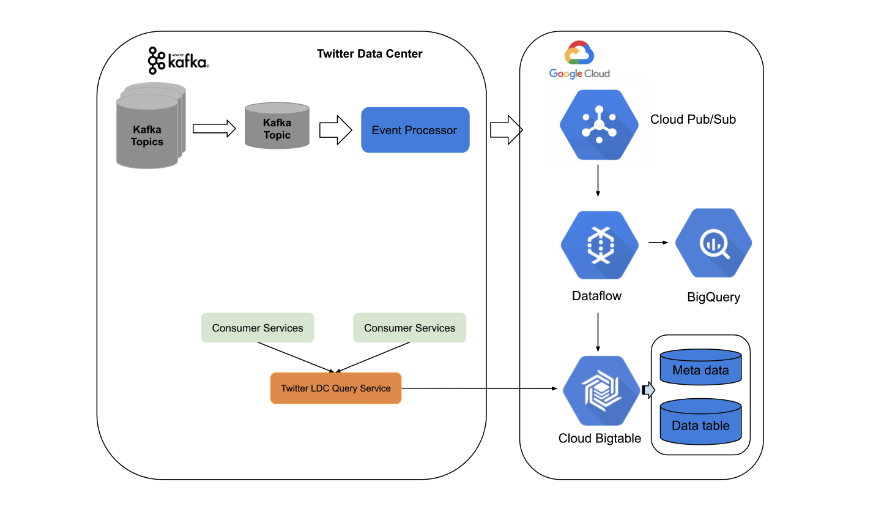
\includegraphics[width=0.9\textwidth]{images/twitter-stack.png}
\caption{Twitter architecture - Kafka and Data Flow}
\label{fig:twitterStack}
\end{figure}

On the twitter data-center the events are preprocessed(transformations and remapping of fields) and will be sent to kafka-topics. On the Google cloud these events are processed and aggrigated in real-time using Twitter internal framework built on top of DataFlow\footnote{https://cloud.google.com/dataflow}. Lastly, the aggregated counts with query keys are written to Bigtable.

\chapter{Conceptual Design}
I propose a simple architecture composed of Apache kafka, Apache spark cluster that can process sentiment of tweets in real-time and dashboard server to visualize results in real-time. The architecture depicted in Fig \ref{fig:application_architecture} shows the conceptual design of my architecture and help us to see the individual components of this project and how they are connected together. The main components are:
\begin{itemize}
  \item Kafka producer
  \item Apache Kafka cluster
  \item Spark cluster(kafka consumer) and
  \item Dashboard web application.
\end{itemize}

\begin{figure}[h]
\centering
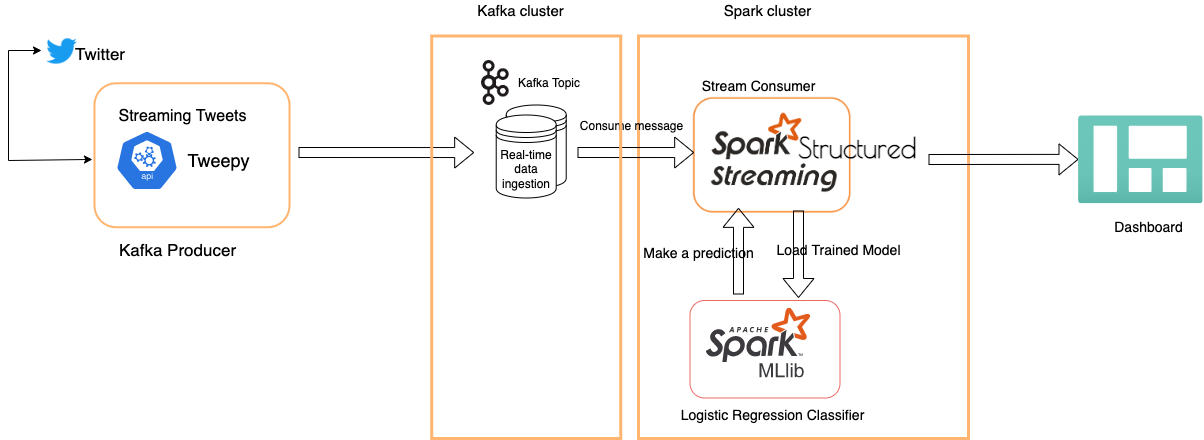
\includegraphics[width=1\textwidth]{images/Tweet sentimenr - architecture.png}
\caption{Overview of Application Architecture}
\label{fig:application_architecture}
\end{figure}

The kafka producer is program that fetches tweets in real-time and publishes to a kafka topic in a kafka cluster. Apache Spark structured streaming will be used to create the processing layer since it offers excellent computational performance in a distributed architecture. This layer will handle all of the basic data processing, such as transformation, aggregation, and sentiment analysis in real-time. We can simply scale horizontally as additional processing power is required because Spark is a distributed computing environment.

\section{Apache Kafka Cluster}
The kafka cluster decouples the communication between stream of tweets(kafka producer) and Spark structured streaming(kafka consumer) allowing us to create multiple producers from different data sources and increase our consumers  to process the streams faster.  
\begin{figure}[h]
\centering
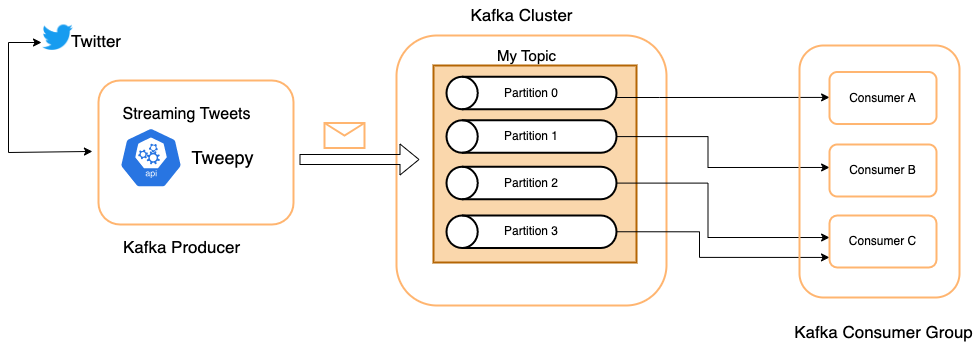
\includegraphics[width=1\textwidth]{images/kafka.png}
\caption{Overview of Kafka workflow diagram}
\label{fig:kafka_architecture}
\end{figure}

The kafka produce request message will be sent from the kafka producer and these messages are stored in the kafka brokers from which the consumer(Spark structured streaming application) will be able to consume the messages and produce the final results.

\section{Apache Spark Cluster}

The spark cluster, depicted on Fig:\ref{fig:application_architecture} acts as a Kafka consumer which run a spark streaming application. The cluster contains driver program and multiple worker nodes. The application is connected to a kafka server and subscribed to on of the "Topics" and continuously receive stream of messages over batches. These batches are processed through different transformations including prediction of sentiments and aggregation to get the total sentiment counts(sentiment prediction count). I have also created another stream that filters out tweets with negative sentiments(filter Negative tweets).  \\

The result from the two streams are sent to the web server via  HTTP POST request to the dashboard server. The dashboard displays total number of tweets processed, total number of tweets with a negative, positive and neutral sentiment and sample of tweets with negative sentiments.

\chapter{Tools exploited}
When designing this system, the main consideration that I took was to design a system that is scalable, fast and that can handle large amounts of stream of data reliably in real-time and efficiently in a fault tolerable fashion. To achieve this design goal I exploited different distributed enabling tools. Lets see them in detail.

\section{Apache Kafka}
Apache Kafka is a distributed  publish-subscribe messaging system. Because stream sizes and velocity changes over time, using Kafka provides the extra benefit of horizontal scaling. Additionally, data segmentation, low latency, and the capacity to manage a large number of different streams are all aspects that makes Kafka a strong fit for the system that I wanted to design. \\

Kafka acts as a data pipeline in my application, providing streaming data. The Kafka producer is built using in python, connects to the Twitter Data API and begins publishing data to Kafka cluster.

\section{Apache Spark: Structured Streaming}

Apache Spark structured streaming is a scalable and fault-tolerant stream processing engine built on the Spark SQL engine. Stream processing applications nowadays requires much faster processing of the data and Spark's resilient distributed dataset (RDD) allows it to speed up computation and transparently keep data in memory and only persist data to a disk what's necessary or to optimize computation.\\

I have used structured streaming to continuously consume messages from the kafka broker and analyse the sentiment of the tweets(messages). Whenever my streaming application starts it loads the model which is persisted on a disk and make the prediction on that.\\

Spark structured streaming does come by default with the package that allows us to read streams from kafka source. For that I have added \textit{org.apache.spark:spark-sql-kafka-0-10\_2.12:3.2.1} package to read the streams.
\section{Apache Spark: Machine Learning Library(MLib)}
MLlib is Apache Spark's scalable machine learning library that is easy to use, scalable and contains many algorithms and utilities\footnote{https://spark.apache.org/mllib/} that makes it easier to combine multiple algorithms into a single pipeline, or workflow. Machine learning classification, regression, clustering and many other algorithms are included in this library. For my purpose since I will be doing sentiment classification I used Logistic regression Estimator to train my sentiment classifier model. MLlib also comes with Estimators which are, as the name suggests are used to evaluate estimator performance metrics over test data.

This library also comes with different utilities that can be used as feature transformation such as standardization, normalization, StopWordRemovers and Tokenizers. I have utilized some of the feature transformers to pre-process the tweet before making the prediction which will be discussed in the implementation section.

Model selection also known as hyperparameter tuning which is a techniques used to find the best model parameters for the given model was performed using tools provided in MLlib\footnote{https://spark.apache.org/docs/latest/ml-tuning.html}. Implementation detail will be provided in the next chapter.

After training, the model has been persisted to a disk to avoid retraining the model all over again. The structured streaming application will be able to load the model and start making the prediction without doing the training again.

\section{John Snow Labs' Spark NLP}

John Snow Labs' Spark NLP is an open source text processing library for Python, Java, and Scala built on top of Apache Spark. It provides production-grade, scalable, and trainable versions of the latest research in natural language processing\footnote{https://www.johnsnowlabs.com/spark-nlp}.\\

I wanted to experiment with this tool because it provides state-of the art feature transformers at scale by extending Apache Spark natively. 

\chapter{Implementation}
In this chapter, I will discuss implementation details and results I achieved from training a classifier model.
\section{Data collection and pre-processing}
For training my model, I collected twitter sentiment dataset from 3 different data sources\footnote{url of the datasets: https://www.kaggle.com/code/kritanjalijain/twitter-sentiment-analysis-lstm}. I collected 182,521 records from these three datasets. The dataset contains two fields, first field is the \textit{text}, representing twets and the second column is \textit{polarity} representing sentiment of the tweet. The \textit{polarity} column has three different values representing the three sentiments. \textbf{0} - Neutral sentiment, \textbf{1} - Positive Sentiment and \textbf{2} - Negative Sentiment. After removing rows with missing values, I ended up with 182329 records. Sentiment distribution is depicted at Table: \ref{tab:svm}
\begin{table}[h]
\centering
    \begin{tabular}{c c c}
        Polarity & Amount \\
        \midrule
        0 & 59111 \\
        1 & 75482 \\
        2 & 47736 \\
        \bottomrule
    \end{tabular}
    \caption{Polarity distribution}
    \label{tab:svm}
\end{table}

I removed usernames and links from the text since these information cannot express any sentiment.

\section{Spark MLlib - Training Model}
To train my model chose Logistic regression classification which is a simple classification algorithm used to predict the probability of a target variable. I experimented with two models and the model has been persisted to disk after training.
\subsection{Logistic regression}
I applied three transformations to convert the text(tweets) to a vector so that it can be used to train my model. The stages are described below.
\begin{figure}[H]
    \centering
    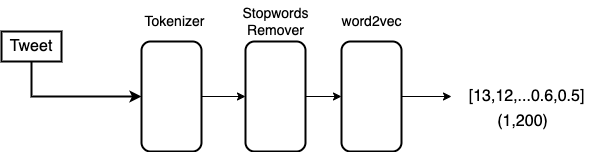
\includegraphics[width=0.6\textwidth]{images/LR.drawio.png}
    \caption{Tweet vectorization stages}
    \label{fig:confusion-svm}
\end{figure}

I used word2vec pre-trained model to convert the tweets to a vector of dimension 200. The dataset has been devided to 85\% for training and 15\% for testing. Additional 20\% of th training set has been reserved for  validation set. I performed model selection over the following hyperparameters.

\begin{table}[h]
\centering
    \begin{tabular}{c c c}
        Parameters & Search space \\
        \midrule
        Tolerance(tol) & $ [0.01, 0.001, 0.0004]$ \\
        Threshold(threshold) & $ [0.4,0.5,0.6]$ \\
        Regularization parameter(regParam) & $ [0.008,0.0008,0.00008]$ \\
        Maximum iteration(maxIter) & $ [1000,5000,10000]$ \\
        \bottomrule
    \end{tabular}
    \caption{Model selection parameters}
    \label{tab:hyperparameter}
\end{table}
I get accuracy of 63\% with best parameters (regParam=0.00008,tol=0.0004,threshold=0.4, maxIter=10000).

\begin{figure}[H]
    \centering
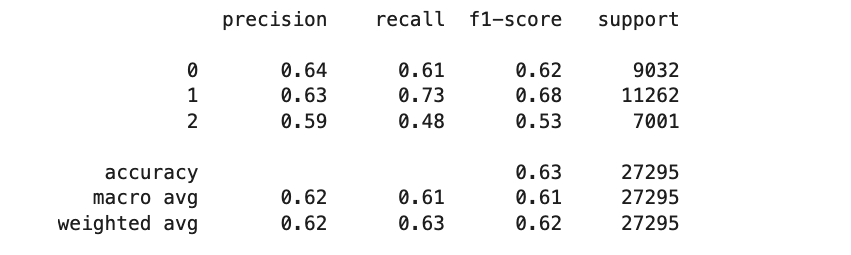
\includegraphics[width=0.9\textwidth]{images/lr.png}
    \caption{Classification result}
    \label{fig:confusion-svm}
\end{figure}

\subsection{Logistic regression with JohnSnow NLP}
JohnSnow NLP provides many state of the art feature transformers. I added some of the transformers to build new feature vectorizer.
\begin{figure}[H]
    \centering
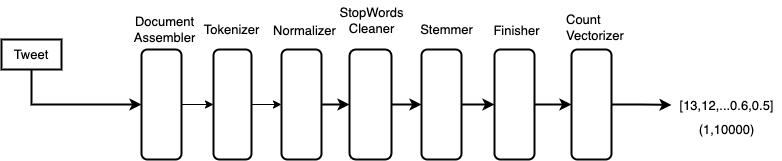
\includegraphics[width=1\textwidth]{images/LR_2.drawio.png}
    \caption{Tweet vectorization stages}
    \label{fig:confusion-svm}
\end{figure}

The documentAssemble prepares the data into a format that is processable by Spark NLP. Then, the tokenizer tokenizes the data and Normalizer is annotator that cleans out tokens. StopWordsCleaner removes the stop words from the tokens and Stemmer converts the token to their root words. Finisher converts annotation results into a format that easier to use. CountVectorizer converts the tokens to a vector. I selected dictionary size of 10000, so the final output will be a vector of size 10000. I performed hyper-parameter search over the parameter specified at Table: \ref{tab:hyperparameter}. These all transformations are based on spark and can be scaled as our data set gets bigger.\\

I get accuracy of 82\% with best parameter (regParam=0.008,tol=0.001,threshold=0.4, maxIter=1000) which significantly better that the previous model. Since the main goal of this project is not getting higher classification accuracy I will use this model to analysis how my spark application perform.

\begin{figure}[H]
    \centering
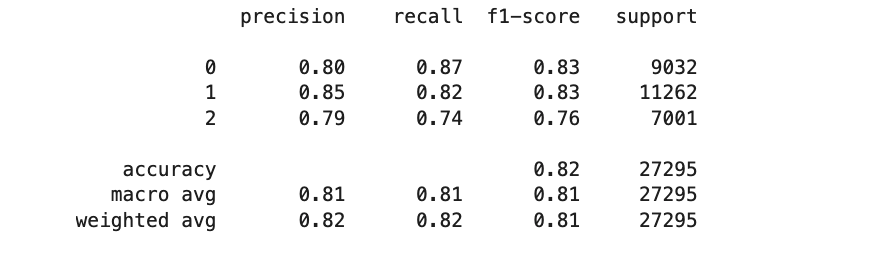
\includegraphics[width=1\textwidth]{images/lr_js.png}
    \caption{Classification result}
    \label{fig:confusion-svm}
\end{figure}

\section{Kafka consumer : Structured streaming}
My kafka consumer is spark structured streaming application. First, it loads the model and start reading the stream from kafka topic. I created two streams, one outputs the total number of counts grouped by sentiments to the sink(sentiment prediction count) and the second outputs negative tweets to the sink(Filter Negative tweets) with \textit{update} output mode. The sink processes each batch and post the results to the dashboard server. The total number of tweets and filtered negative tweets are sent to the dashboard server for visualization. 

\section{Kafka producer : Tweepy}

I utilized Tweepy\footnote{https://github.com/tweepy/tweepy}, an easy-to-use Python library for accessing the Twitter API that lets us to integrate the Twitter API into our Kafka Producer, to stream data from the Twitter API to Kafka topic. The Twitter requests fetched from from Twitter API are packaged into a kafka producer record with specified topic(in my case, \textbf{Elon Musk}). Then the producer serializes and partitions the message and will be will be sent in a batch to a partition leader. Ultimately the partition leader will send the message the "kafka consumer". I used \textit{json\_serializer} as a value serializer and I didn't use key for the topic.\\

 Twitter allows to fetch maximum of 100 results per single request with \textbf{Essential} access level. I collected \textit{date created}, \textit{text}(tweet text),\textit{tweet id}, \textit{username} and \textit{profile url} informations. It took on average 0.65 seconds to process one request and publish to kafka.
 
\section{Dashboard server}
The dashboard server is a web app built using flask. On the dash we can monitor total number of tweets processed, positive tweets, negative tweets and neutral tweets. Additionally, recent negative tweets are continuously displayed on the dashboard.

\begin{figure}[H]
    \centering
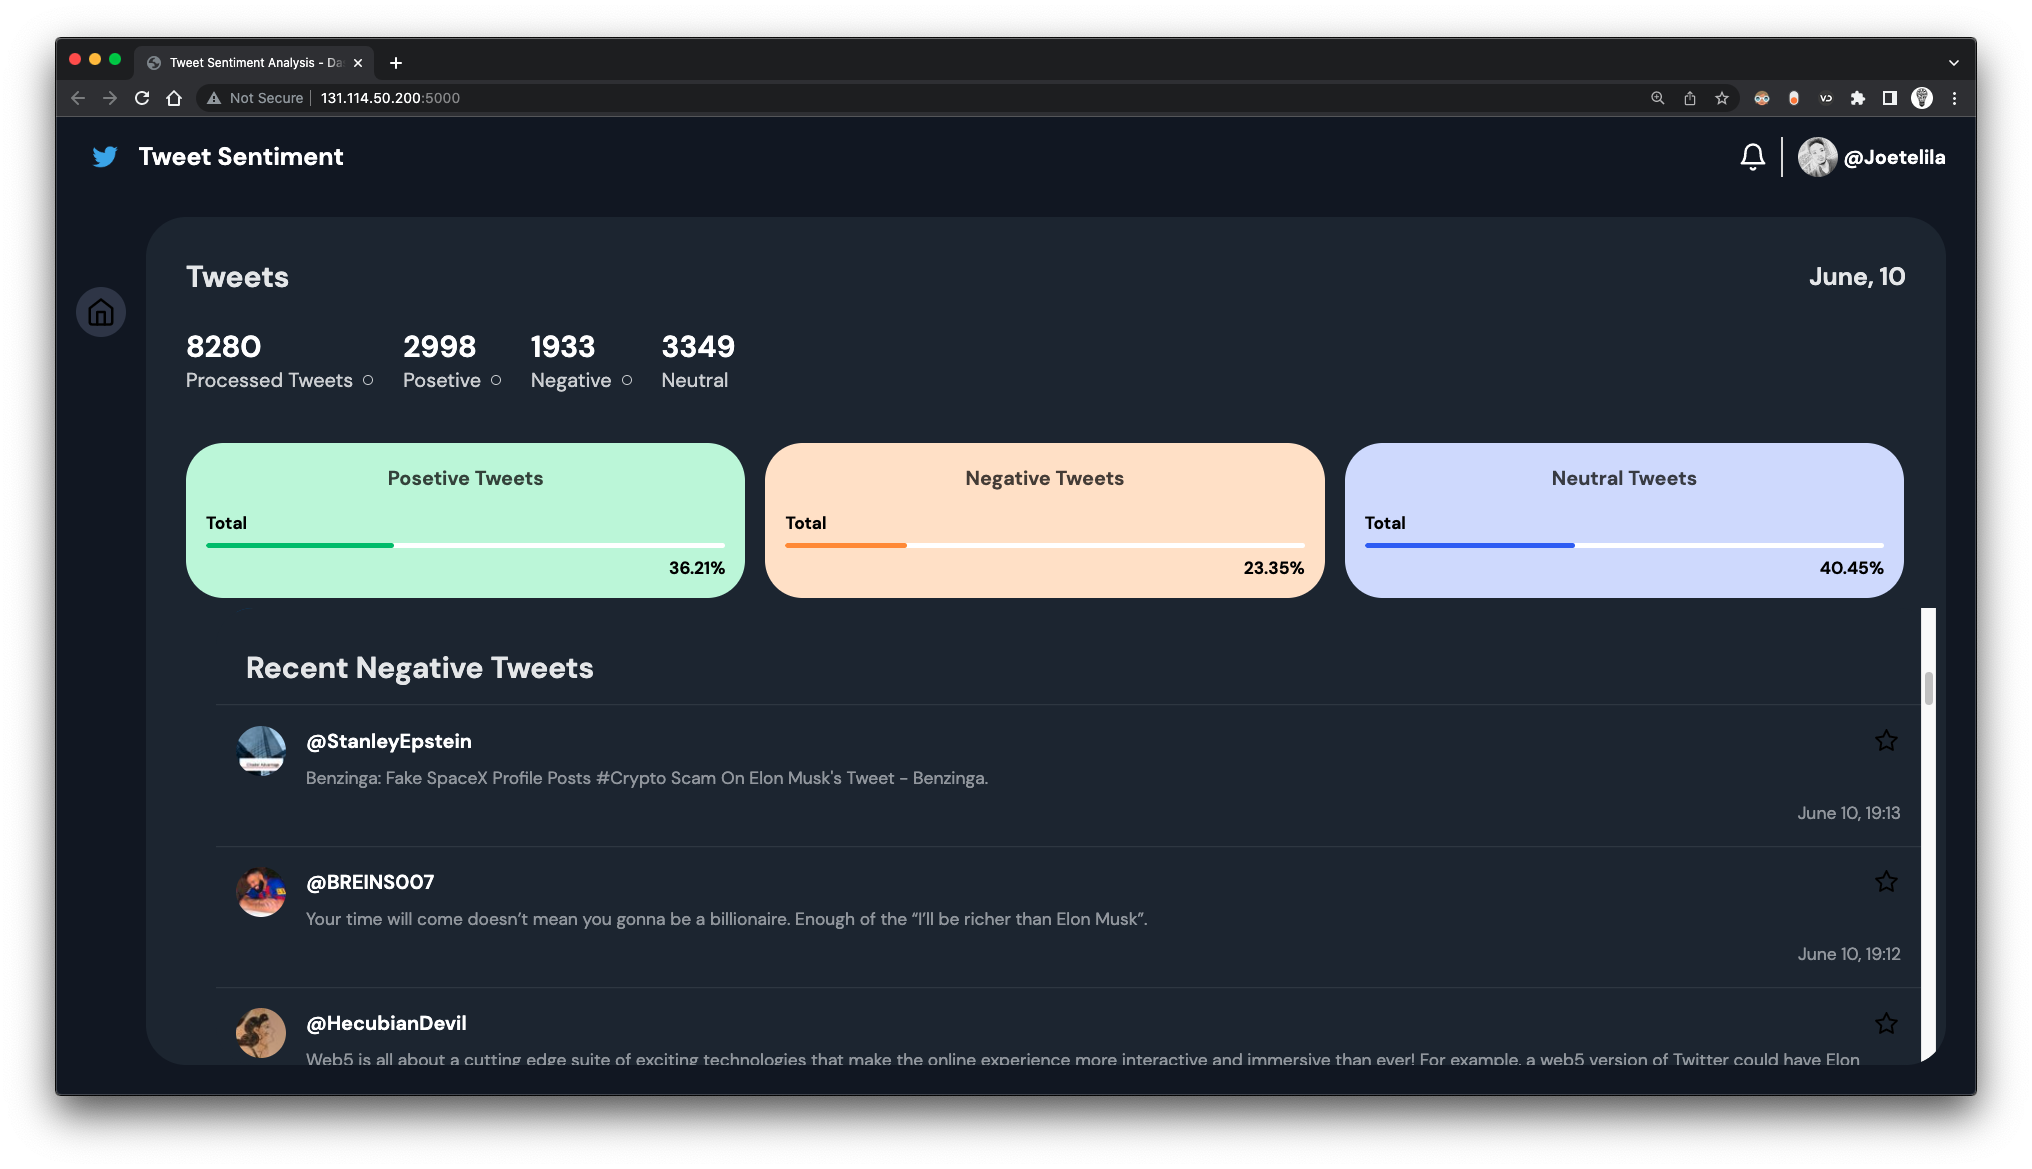
\includegraphics[width=0.9\textwidth]{images/dashboardss.png}
    \caption{Classification result}
    \label{fig:confusion-svm}
\end{figure}

\chapter{Experiments}
\section{Environment setup and measurements}
All the experiments are performed on a remote cluster machines provided to us. The driver machine is Intel(R) Xeon(R) Gold 5218 CPU @ 2.30GHz with 4 cores and has 32GB of RAM. The worker node is also Intel(R) Xeon(R) Gold 5218 CPU @ 2.30GHz but with 2 cores and 8GB of memory. In total we have 8 worker nodes and 1 driver node.

I performed my experiment by changing the number of worker nodes and analysing 4 key measurements. These measurements are collected from Streaming Query Statistics page of spark ui \cite{sparkAnalysis}.

\begin{itemize}
   \item \verb|Input rate(rec/sec): | Represents rate at which data is arriving.
   \item \verb|Process rate(rec/sec): | Rate at which spark is processing data.
   \item \verb|Input rows(rec): | Represent the number of records processed in a trigger.
   \item \verb|Batch duration(msec): | The duration at which each batch is being processed.
\end{itemize}

The experiment is performed under two scenarios. The first scenario uses only two workers and the second scenario uses all 8 workers. The result is discussed in the next section.
\section{Results}
I performed the query as fast as feasible to handle Apache Kafka data. The streaming task will process all accessible data in Kafka for each batch. The \textbf{Input rate} is in the range of \textbf{100-150 records/sec} in all scenarios which is quite reasonable given the fact that the kafka is producing at the rate \textbf{150 records/sec}.\\

\begin{figure}[H]
    \centering
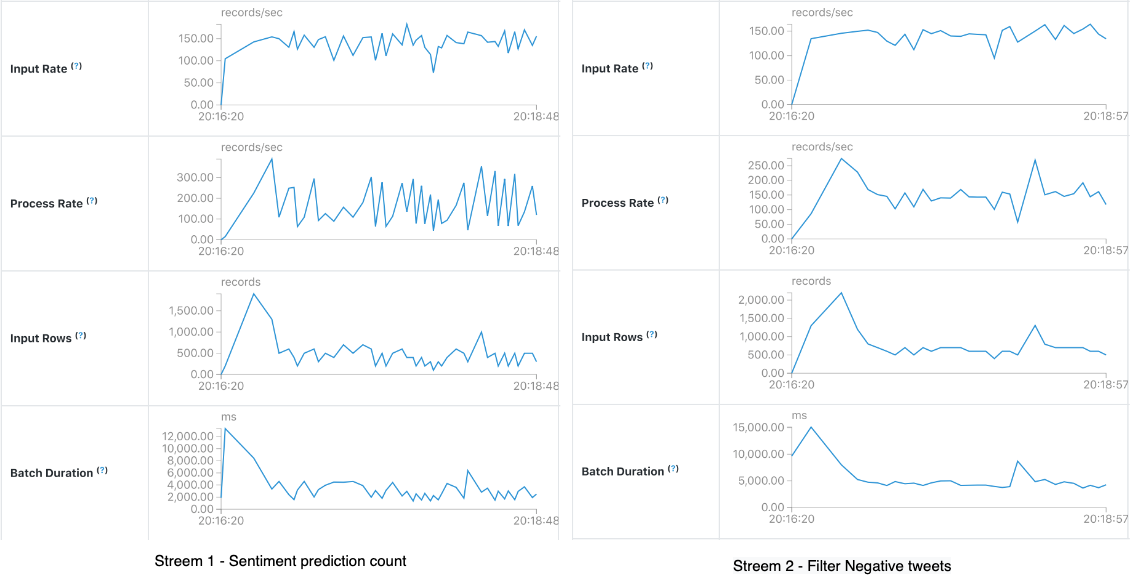
\includegraphics[width=1\textwidth]{images/worker2results.drawio.png}
    \caption{Scenario1: Stream result from 2 worker nodes}
    \label{fig:workers2}
\end{figure}

From the \textbf{process rate} we can understand that spark is able to process at the rate at which data is arriving in both scenarios and streams. This means the \textbf{input rate} is smaller than what the spark stream can able to process. 

\begin{figure}[H]
    \centering
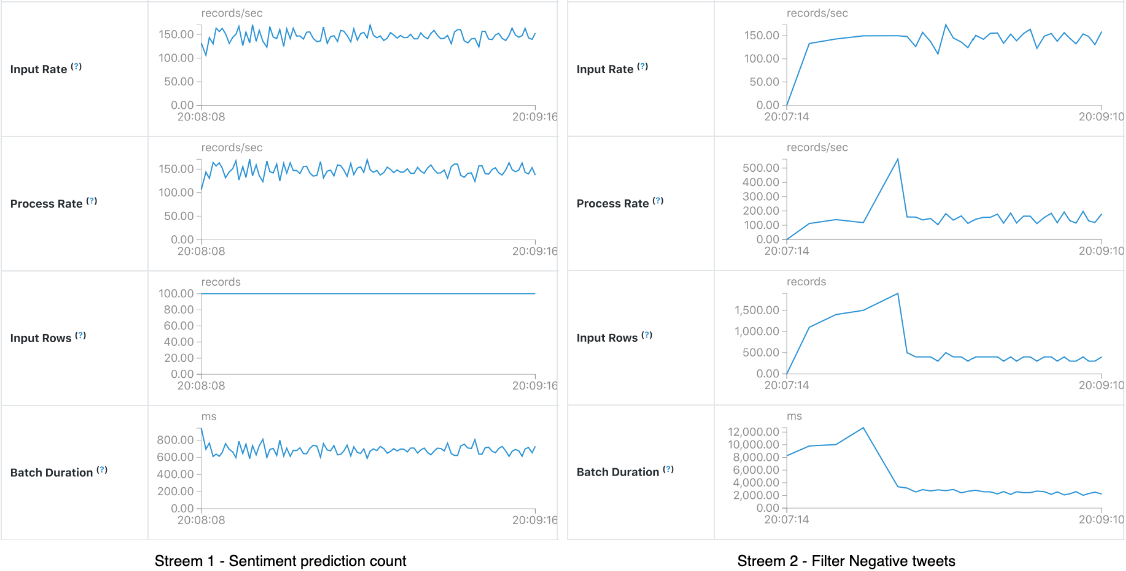
\includegraphics[width=1\textwidth]{images/worker8result.drawio.png}
    \caption{scenario2: Stream result from 8 worker nodes}
    \label{fig:workers8}
\end{figure}

The main difference we can notice in both scenario is in \textbf{batch duration}. Intuitively, if the stream processing capacity of cluster is not enough, the \textbf{batch duration} or latency will rise. Scenario1 is in the range of 2-4 seconds for stream1, some batches even taking longer than 4 seconds and 5 seconds in stream2. The main reason for this would be higher number of records in a batch or less number of resources to process the data and we can decrease this time by adding more resources to the cluster. We can observe this on the second scenario where the \textbf{batch duration} is in the range of 0.6-0.8 second in stream1 and 2 seconds in stream2 - much better improvement. Indicating spark can be able to process much bigger \textbf{Input rate}.

\section{Conclusion}
This report has described an approach to perform sentiment analysis based on Apache Spark, Kafka, and MLlib, scalable frameworkds. Using spark cluster I was able process realtime tweets efficiently. The most important fact is that this system can adapt to the changing amount of streams. If the input rate gets bigger, we can add more consumer to the topic without making significant change to the code or if the rate gets smaller, we can remove some workers or decrease the resource of our cluster so that we don't waste processing power. \\

Finally, I was able to understand the principles of distributed systems as a result of this project. Implementing this application to analyze real-time sentiment taught me how to utilize Spark to address large data and stream problems.


\section{Folder structure and how to run the code}
The project folder \textbf{Sentiment-analysis-using-kafka-spark-final} contains three sub-folders. \textbf{dashboardServer} folder contains the implementation for web dashboard server. \textbf{data} folder contains the data used for training. \textbf{pipeline\_lr\_js\_model}(logistic regression with transformation from johnsnowlab) and \textbf{pipeline\_lr\_model} are the two models persisted on a disk. \textbf{Report} folder contains this report files.\\

To run the project first, start kafka zookeeper and kafka server.

\begin{minted}{bash}
#!/bin/bash
$ zookeeper-server-start.sh config/zookeeper.properties
\end{minted}

\begin{minted}{bash}
#!/bin/bash
$ kafka-server-start.sh config/server.properties
\end{minted}

Then, create a kafka topic with 5 partitions.
\begin{minted}{bash}
#!/bin/bash
$ kafka-topics.sh --create --bootstrap-server 131.114.50.200:9092 \
--partitions 5 --topic ElonMusk 
\end{minted}

Next, launch kafka producer.

\begin{minted}{bash}
#!/bin/bash
$ python3 /kafka-script/tweet_producer.py 
\end{minted}

Now we are ready to submit our spark job.

\begin{minted}{bash}
#!/bin/bash
$ spark-submit --packages org.apache.spark:spark-sql-kafka-0-10_2.12:3.2.1,\
                 com.johnsnowlabs.nlp:spark-nlp_2.12:3.4.4  \
                --master spark://131.114.50.200:7079 \ 
                 kafka-script/tweet_consumer.py 
\end{minted}

Finally, launch web dashboard server using below command inside \textit{dashboardServer} folder.

\begin{minted}{bash}
#!/bin/bash
$ flask run -h 131.114.50.200 
\end{minted}

\medskip
\printbibliography

\end{document}